\documentclass[12pt,oneside]{article}
\usepackage[utf8]{inputenc}
\usepackage{float}
\usepackage[bottom]{footmisc}
\usepackage{bookmark}
\usepackage{microtype}
\usepackage{amsmath}
\usepackage{multicol}
\usepackage{mdframed}
\usepackage{setspace}
\usepackage{pgfplots}
\usepackage{graphicx}
\usepackage{fancyvrb}
\usepackage[absolute]{textpos}\TPGrid{16}{16}
\usepackage{tikz}
  \usetikzlibrary{shapes}
  \usetikzlibrary{arrows.meta}
  \usetikzlibrary{arrows}
  \usetikzlibrary{shadows}
  \usetikzlibrary{trees}
  \usetikzlibrary{fit}
  \usetikzlibrary{calc}
  \usetikzlibrary{positioning}
  \usetikzlibrary{decorations.pathmorphing}
\usepackage{./tikz-uml}
\usepackage{everypage}
  \AddEverypageHook{
    \begin{textblock}{0.5}[0,0](0,0)
      \tikz \node[fill=mypink,minimum width=0.5\TPHorizModule,minimum height=16\TPVertModule] {};
    \end{textblock}
    \begin{textblock}{0.125}[0,0](0.5,0)
      \tikz \node[fill=myblack,inner sep=0, minimum width=0.125\TPHorizModule,minimum height=16\TPVertModule] {};
    \end{textblock}
  }
\usepackage{xcolor}
  \definecolor{firebrick}{HTML}{B22222}
  \definecolor{myred}{HTML}{CF0A2C}
  \definecolor{mypink}{HTML}{560CCE}
  \definecolor{myblack}{HTML}{232527}
\newcommand\dd[1]{\colorbox{gray!30}{\texttt{#1}}}
\usepackage{hyperref}
  \hypersetup{colorlinks=true,allcolors=blue!40!black}
\setlength{\topskip}{6pt}
\setlength{\parindent}{0pt} % indent first line
\setlength{\parskip}{6pt} % before par
% \let\oldsection\section\renewcommand\section{\newpage\oldsection}
\date{\small\today}
\title{%
  MkDrop: Tokens Flow Management\\
  \colorbox{mypink}{\small\sffamily\color{white}{White Paper}}}
\usepackage[style=authoryear,sorting=nyt,backend=biber,
  hyperref=true,abbreviate=true,
  maxcitenames=1,maxbibnames=1]{biblatex}
  \renewbibmacro{in:}{}
  \addbibresource{books.bib}
\tikzset{node distance=1.6cm, auto, every text node part/.style={align=center, font={\sffamily\small}}}
\tikzstyle{block} = [draw=myblack, fill=white, inner sep=0.3cm, outer sep=0.1cm, thick]
\tikzstyle{ln} = [draw, ->, very thick, arrows={-triangle 90}, every text node part/.append style={font={\sffamily\scriptsize}}]
\author{Bohdan Snisar \and Yurii Chudinov} % Add authors here
\begin{document}
\raggedbottom

\maketitle
\begin{abstract}
  In the rapidly evolving landscape of cryptocurrency, the distribution of tokens, particularly through airdrops, 
  plays a pivotal role in project promotion and community engagement. However, the current methods for token 
  distribution   are fraught with challenges like high transaction costs, security risks, and inefficient processes. 
  This white paper proposes a novel platform designed to streamline and secure the process of token distribution 
  while maintaining the anonymity characteristic of the post crypto world.
\end{abstract}

% \onehalfspace

\section{Introduction}

The rapidly expanding cryptocurrency sector relies heavily on effective token distribution,
crucial for engaging and maintaining community support. \cite{ziegler2023navigating} This white paper introduces an innovative 
platform designed to optimize token distribution processes, enhance security, and foster authentic 
community growth. Token distribution, essential for allocating digital assets to stakeholders like investors, 
team members, and users, has evolved to reflect the dynamic and complex nature of the cryptocurrency world. \cite{Fan_2023}

\begin{description}
  \item[Initial Coin Offerings (ICOs)]
  Since their emergence in 2013, Initial Coin Offerings (ICOs) have become a favored funding 
  method for crypto projects. Investors contribute assets such as Bitcoin to early developers, 
  receiving tokens in return at the network's launch. This method gained popularity with major projects 
  like Ethereum raising significant funds through ICOs.

  \item[Venture Capital Investment]
  In this traditional approach, venture capitalist firms invest in crypto startups by 
  purchasing their tokens, distinct from typical venture capital which focuses on acquiring company equity.

  \item[Airdrops]
  Airdrops are utilized as a marketing tool to distribute a limited number of 
  tokens directly to user wallets. This strategy is instrumental in increasing awareness 
  of the project and building a network effect.

  \item[Lockdrops]
  Lockdrops are an innovative distribution method where users temporarily lock up their existing 
  tokens before the introduction of a new cryptocurrency. This model is based on the participants' 
  commitment to the new project's success.

  \item[Public Sales]
  This category encompasses methods like Initial Exchange Offerings (IEOs) and Initial DEX Offerings
  (IDOs). Here, tokens are released into the market through exchanges, offering a decentralized way 
  of distributing tokens.
\end{description}


\section{Challanges}

In the ever-evolving landscape of cryptocurrency ventures, the implementation of token vesting schedules is 
a crucial factor that requires thoughtful planning. Once these schedules are embedded in smart contracts, 
they become permanent. This permanence guarantees transparency and fosters trust, but it also adds a degree 
of inflexibility. \cite{liu2022fighting} This can be particularly problematic for projects that are still refining their strategies. \cite{messias2023airdrops}

\begin{description}
  \item[Challenges to Project Adaptability]
  In the early and frequently changing stages of cryptocurrency projects, the unalterable nature 
  of vesting schedules fixed in smart contracts can cause a disconnect. This misalignment happens 
  between the project's evolving needs and the predetermined plans for token distribution.

  \item[Confidence]
  Stakeholder trust can be deeply affected if there are significant changes in the project's direction
  after the initial token distribution or airdrop. Unchangeable vesting schedules might leave stakeholders 
  feeling unfairly treated, which can impact their continued support and confidence in the project.

  \item[Operational and Strategic Flexibility]
  Rigid vesting schedules can restrict the project team's capability to adjust strategies. 
  This limitation affects various aspects such as modifying the project's scope, extending development 
  timelines, or shifting the project's strategy in response to market feedback, technological developments, 
  or shifts in the project's ecosystem.
\end{description}


\section{Solution}

The "Provisional Token Allocation" approach involves initially reserving tokens for users without 
directly allocating them to their wallets. 

Instead, users are provided with placeholders or "slots" representing their entitlement to tokens. 
These slots remain provisional until certain criteria or milestones are met, at which point 
the tokens are materialized or converted into immutable tokens. 

The criteria for materialization 
can vary, including project milestones, market conditions, or predefined time-based factors. 
This approach offers flexibility in the timing of token distribution.

Keynotes from the process flow:
\begin{enumerate}
  \item \textbf{Token Allocation by Company:} The starting point where the company determines and allocates tokens.
  \item \textbf{Wallet Verification:} Users undergo a verification process to ensure uniqueness. 
  Uniqueness must satisfy only proof of \textbf{one user} == \textbf{one wallet} and not aim to 
  reveal users’ identities.
  \item \textbf{Provision:} Users claim their tokens, resulting in the assignment of ’provisional’ tokens. Such tokens signify a placeholder for future
  and just exist on user wallets as slots.
  \item \textbf{Materialization:} The provisional tokens are materialized into actual tokens. Materialization 
  means linking them from a placeholder contract to a real smart contract, embedding business 
  logic such as vesting and other features. By its nature, this process follows the intuition 
  of \href{https://en.wikipedia.org/wiki/Late_binding} a well-known concept in software development. 
  \item \textbf{Distribution:} The actual tokens are then distributed to the end users.
\end{enumerate}

\begin{figure}[H]
  \centering
  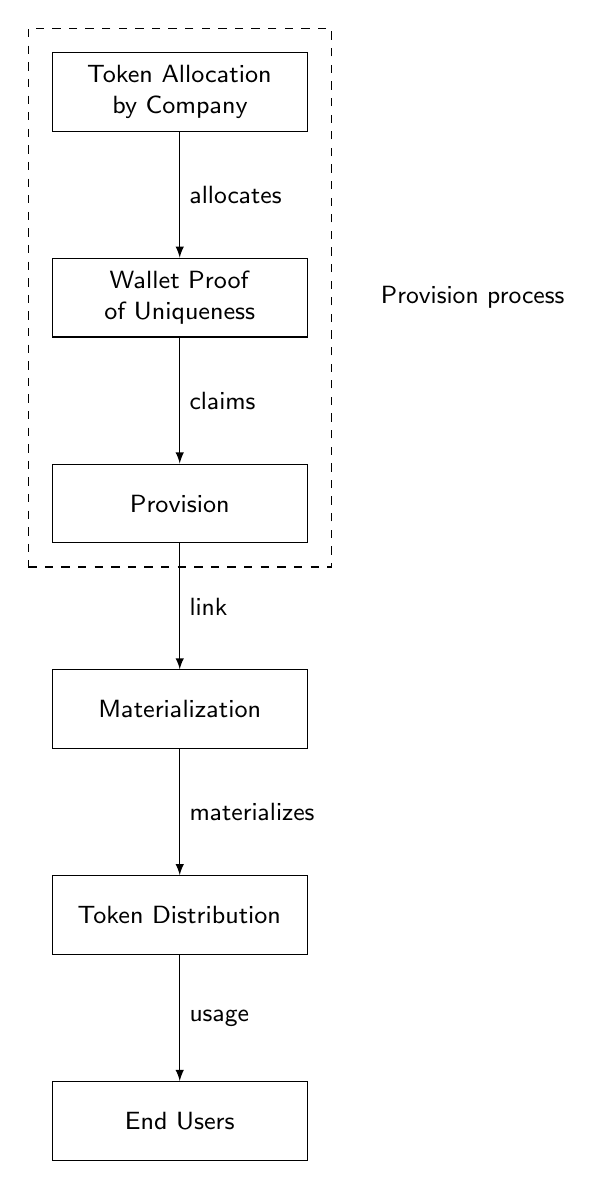
\begin{tikzpicture}[block/.style={rectangle, draw, text width=3cm, align=center, minimum height=1cm}, >=latex]
    % Nodes
    \node[block] (alloc) {Token Allocation by Company};
    \node[block, below=of alloc] (verify) {Wallet Proof of Uniqueness};
    \node[block, below=of verify] (provision) {Provision};

    % Dashed container with description
    \node[fit=(alloc)(verify)(provision), dashed, draw, inner sep=0.3cm] (container) {};
    \node[right=0.5cm of container] {Provision process}; % Label on the right

    \node[block, below=of provision] (materialize) {Materialization};
    \node[block, below=of materialize] (distribution) {Token Distribution};
    \node[block, below=of distribution] (users) {End Users};
  
    % Paths
    \draw[->] (alloc) -- node[right] {allocates} (verify);
    \draw[->] (verify) -- node[right] {claims} (provision);
    \draw[->] (provision) -- node[right] {link} (materialize);
    \draw[->] (materialize) -- node[right] {materializes} (distribution);
    \draw[->] (distribution) -- node[right] {usage} (users);
  \end{tikzpicture}
  \caption{Token Allocation Process with Provisional Tokens.}
  \label{fig:token_allocation_prov}
\end{figure}


\section{Requirements}
\label{sec:requirements}

Token distribution, traditionally solved through specific smart contracts for distribution or vesting, often involves complex and costly alterations due to code-level 
vesting and locking. However, alternative distribution methods exist:
\begin{itemize}
  \item Custodial Solutions: Centralized entities like crypto exchanges handle airdrop vesting, managing token storage and distribution.
  \item Multisignature Wallets: These wallets require multiple approvals for transactions, offering a decentralized approach to managing vesting.
\end{itemize}
Each method addresses certain issues but has limitations.

\subsection{Features}
\label{sec:features}

The crypto community expects an airdrop platform to exhibit
several key qualities and features. The most crucial functional
requirements are:

\begin{description}
  \item[Claim Token Creation]
  Users can create a claim token directly on their devices, enabling airdrop requests without on-chain transactions. This token, a hashed hardware fingerprint, is generated on-device and contains no personal data.

  \item[Digital Profile]
  Utilizing the digital fingerprint, users can create anonymous profiles for social network integration and subscription management, facilitating community interaction.

  \item[Human-Proof Approach]
  To counter artificial identities, backup codes or claim-token restoration processes incorporate human verification, enabling token and profile transfers between devices.

  \item[Asset Provisioning]
  The platform provides a mechanism for secure token or crypto asset distribution, facilitating flexible adjustments in vesting conditions or coin operations.

  \item[Token Flow Automation]
  Automating token distribution reduces manual involvement, significantly lowering operational costs associated with community management.
\end{description}

\subsection{Non-functional Requirements}
\label{sec:nfr}

The most important \href{https://en.wikipedia.org/wiki/Non-functional_requirement}{non-functional requirements} are:

\begin{description}
  \item[Security]
  This is paramount in blockchain systems to protect against fraud, hacks,
   and unauthorized access. Security measures could include multi-factor authentication, 
  encryption, secure smart contract coding practices, and regular security audits

  \item[Scalability]
  The system should be able to handle increasing workloads and 
  accommodate growth in user numbers and transaction volumes. Potential rarer but peak volumes during short timeframe.  
  This might involve off-chain processing claims, optimizing smart contract efficiency,
  considering layer 2 scaling solutions, or implementing sharding techniques

  \item[Cost Efficiency]
  Managing transaction costs, especially on networks with high gas fees, 
  is crucial for both the users and the company. 
  Optimizing smart contract execution and considering gas-efficient 
  algorithms are important in this regard.

  \item[Flexibility]
  System must satisfy main needs of crypto projects in 2 dimentions: 
  token governance and community management.

\end{description}

\section{Architecture}
Architecure is consisted of several essential parts:

\begin{description}
  \item[Hand Print] 
  Hand prints are used to ensure each user's device is unique. This method involves checking unique features of a user's device to prevent multiple accounts or duplications. It's a reliable way to make sure every device is linked to a specific user, which is crucial for securing access to web3 wallets and transactions. 
  
  \begin{enumerate}
      \item \textbf{Multi-Factor Authentication (MFA)}: MFA adds layers of security by requiring different forms of verification, such as passwords, devices, or biometric data.
      \item \textbf{Passkeys}: Passkeys replace traditional passwords with device-specific keys, increasing security by keeping sensitive data off the network.
      \item \textbf{One-Time Passwords (OTP)}: OTPs are temporary codes sent to a user's device, adding an extra step of verification to ensure the person accessing the account is the legitimate owner.
  \end{enumerate}  

  \item[Provision]
  The Provision process in our system takes place off-chain, ensuring
  efficient and cost-effective operation. It starts when a user generates a unique proof of
  device identity and submits this data to an Oracle. The Oracle's key role is to verify this uniqueness 
  against a nullifier, a mechanism to ensure that each proof is distinct and hasn't been used before. 
  If the proof is indeed unique, the Oracle generates provision codes, which are essentially tokens allocated 
  to the user. These provision tokens are stored within the Oracle, making the process gas-free since it doesn't require
  on-chain transactions. This approach not only enhances efficiency but also significantly reduces costs associated with
  on-chain operations, making it an ideal solution for scalable and user-friendly web3 applications before airdrop activity.

  \item[Nullifier]
  A nullifier in our system is a cryptographic marker used to prevent duplicate claims or actions. 
  Based on Semaphore \href{https://semaphore.pse.dev/} as a zero-knowledge protocol that allows to cast a message (endorsement in this case).
  It's a key element for user privacy and security, allowing action verification without revealing 
  user identities. \cite{semaphore_pse_dev}

  \item[Provision]
  The Provision process offers an innovative approach for companies to initiate token-related activities without needing an existing ERC-20 coin. 
  This method enables the creation of provisional tokens, 
  which act as placeholders for future real tokens. It's particularly useful for companies in the early stages of their project, allowing them to engage in 
  activities like community incentives or preliminary token distribution, with the actual ERC-20 tokens to be issued later on. Provision thus offers flexibility and agility in
  managing token-based operations, even before the official minting of ERC-20 coins.

  \item[Allocate]
  The Allocate process allows companies to fund 
  their activities by transferring ERC-20 tokens to the 
  Budget Golem contract. This straightforward method 
  centralizes company tokens in one contract, streamlining 
  the management of token-based operations like airdrops or incentives.
  This approach can be treated as Later Binding when provision slots of Airdrop are linked with real contracts that encapsulate tokenomic, casting, and other specifics.
\end{description}


\begin{figure}[H]
\centering
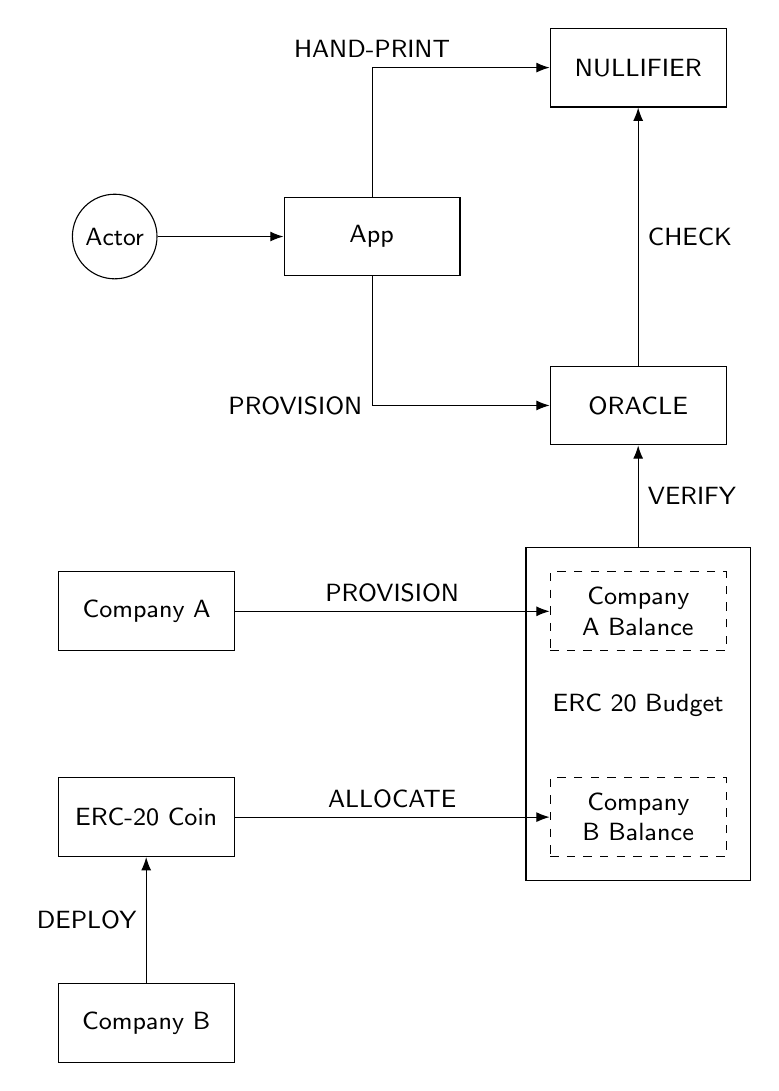
\begin{tikzpicture}[
    block/.style={rectangle, draw, text width=2cm, align=center, minimum height=1cm},
    line/.style={draw, -Latex}
  ]

  % Define actor
  \node[circle, draw] (actor) {Actor};

  % Define app block
  \node[block, right=of actor] (app) {App};

  % Define nullifier and oracle blocks
  \node[block, above right=of app] (nullifier) {NULLIFIER};
  \node[block, below right=of app] (oracle) {ORACLE};

  % Define ERC-20 related blocks
  % \node[block, below=of oracle] (erc20) {ERC-20 Budget};
  \node[block, dashed, below=of oracle] (companyA) {Company A Balance};
  \node[block, dashed, below=of companyA] (companyB) {Company B Balance};
  \node[fit=(companyA)(companyB), draw, inner sep=0.3cm] (erc20) {ERC 20 Budget};

  % Define Inputs
  \node[block, left=4cm of companyA] (companyACoin) {Company A};
  \node[block, left=4cm of companyB] (companyB_ERC20) {ERC-20 Coin};
  \node[block, below=of companyB_ERC20] (compnayBCoin) {Company B};

  % Draw lines
  \draw[line] (actor) -- (app);
  \draw[line] (app) |- (nullifier) node[midway, above] {HAND-PRINT};
  \draw[line] (app) |- (oracle) node[midway, left] {PROVISION};
  \draw[line] (oracle) -- (nullifier) node[midway, right] {CHECK};
  \draw[line] (erc20) -- (oracle) node[midway, right] {VERIFY};

  \draw[line] (companyACoin) -- (companyA) node[midway, above] {PROVISION};
  \draw[line] (companyB_ERC20) -- (companyB) node[midway, above] {ALLOCATE};
  \draw[line] (compnayBCoin) -- (companyB_ERC20) node[midway, left] {DEPLOY};
  
\end{tikzpicture}
\caption{Architecture Overview}
\label{fig:arch}
\end{figure}


\section{Extensions}
This document aims to outline a solution that revolutionizes 
the distribution of coins within the web3 framework. We're seeking 
to develop an innovative system that not only simplifies the process 
of token distribution but also addresses the inherent challenges of the 
current methodologies, such as cost inefficiency, 
lack of flexibility, and complex management requirements. 

\section{Acknowledgements}
\label{sec:ack}

The document was originally created by Yurii Chudinov and Bohdan Snisar. 

\printbibliography%
\end{document}
